\section{Programm}
\subsection{Einleitung}
Um die Methoden der Threads in einer Realen Situation zu nutzen, habe ich mich entschlossen ein Programm, welches stark von Threads profitieren kann, zu programmieren.  

Ich habe mich für ein Programm eintscheiden, mit dem man ein Bild mit vielen weiteren Bildern rekrieren kann. Es wird demnach ein Mosaik aus Bildern erstellt.

\begin{figure}[h]
    \centering
    \subfloat[\centering Input]{
        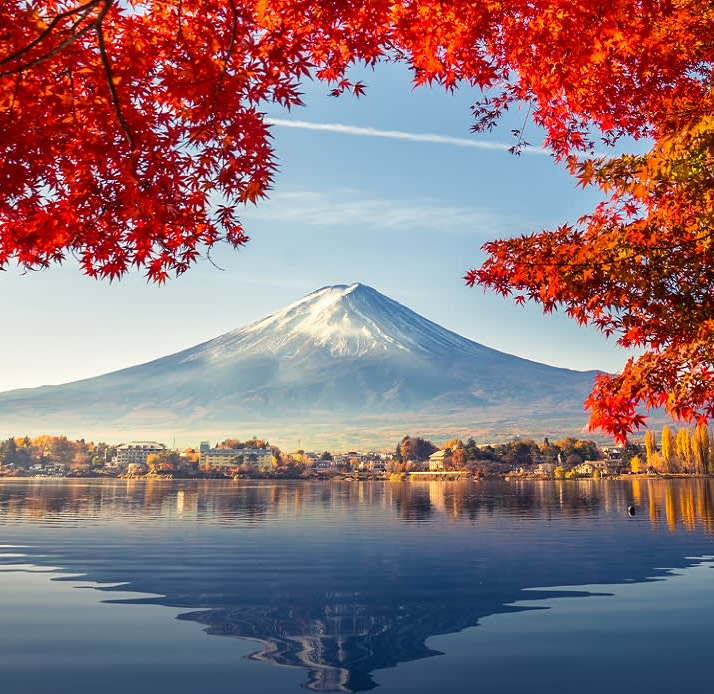
\includegraphics[height=5cm]{images/Source_100x100}
    }
    \subfloat[\centering Output]{
        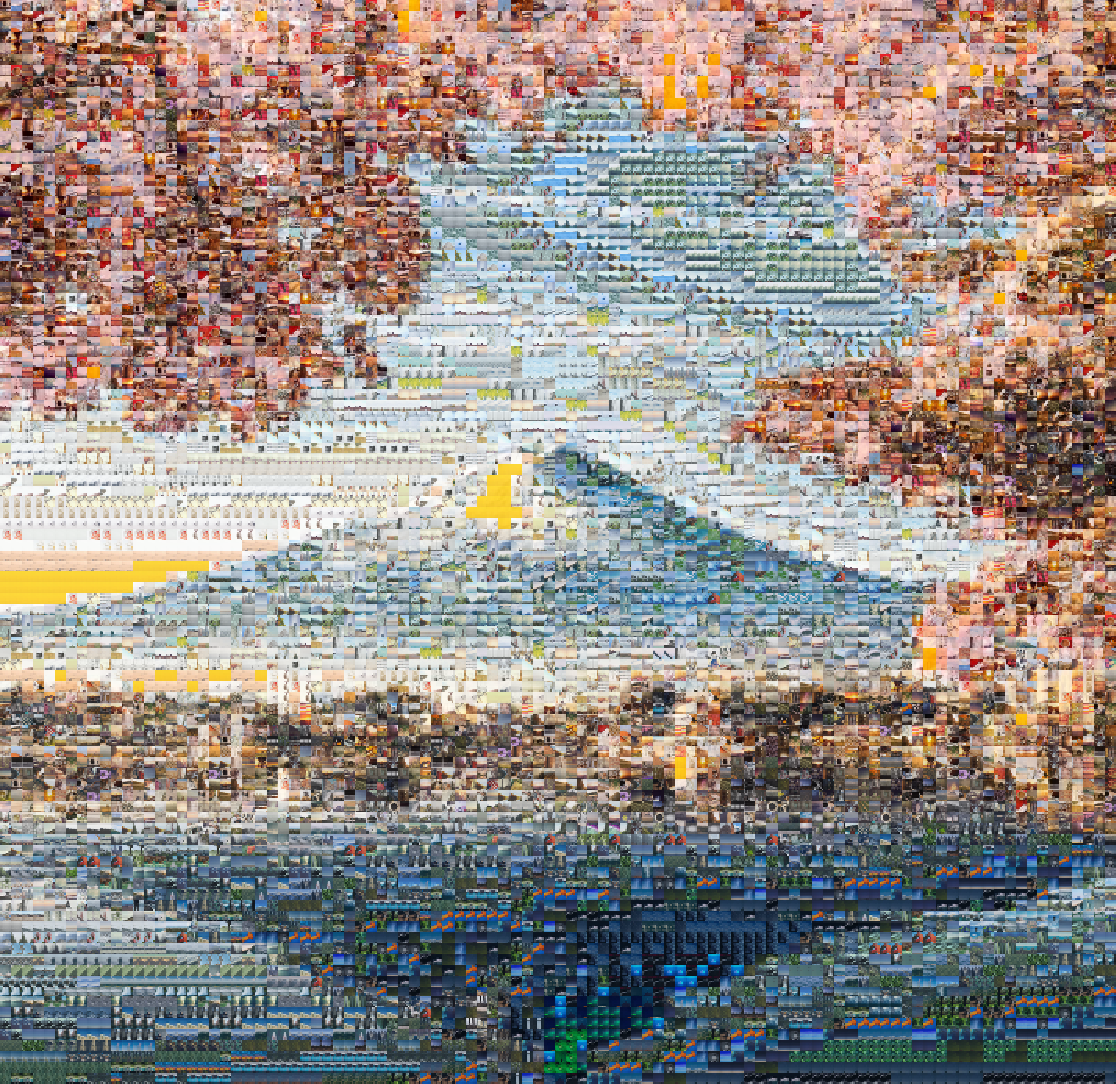
\includegraphics[height=5cm]{images/Render_100x100}
    }
    \caption[Programm Funktion]{Funktionsweise des Programmes}
\end{figure}

Die anwendung von Threads kommt in dem Programm in vielen Stellen vor. Im folgen werde ich mich auf den Algorythmus der Bild analyse und verarbeitung beziehen. Andere aspekte, wie die implementation des Testmodus und andere Features, die in der App vorhanden sind, werden kurz im Anhang erwähnt.

\newpage
\subsection{Idee}
In der genaueren Betrachtung, muss das Programm das eingegebene Bild vereinfachen. Dies wird durch eine Unterteilung des Bildes in Sektoren erreicht. Die Sektoren sind auch die zukünftigen Stellen für die ausgewählten Bilder. Es wird die durchschnittliche Farbe der Sektoren berechnet. Das selbe vorgehen wird auch auf die ausgewählten Bilder angewendet. Dabei ist ein Bild ein Sektor. Dieses vorgehen erlaubt es auch, Datenbanken (im JSON-Format) zu erstellen, da sich die durchschnittliche Farbe der ausgewählten Bilder nicht ändern wird. Anschließend wird mit einem Algorithmus die passenden Bilder für die einzelnen Sektoren berechnet. Dabei unterliegt der Algorithmus der Beschrenkung, dass der Nutzer wählen kann, wie häufig ein Bild vorkommen darf. Nach dem berechnen der benötigten Bilder müssen diese für die Verwendung angepasst werden. Es soll schließlich nicht ein 10x10px großer Teil aus einem 4000x3000px Bild verwendet werden. Dazu wird das Bild erst Skaliert und schließlich zurechtgeschnitten. Dabei liegt der Fokus darauf, immer die Mitte des Bildes zu treffen. Das Programm arbeitet die Schritte nachfolgend ab und in dieser Reihenfolge werde ich das Programm nachfolgend erklären.

\subsection{Implementation in Java}
\subsubsection{Berechnen der Sektionen}
Das berechnen der Sektionen ist eigentlich ziemlich geradeaus. Die Größe des Bildes ist bekannt und in wie viele Teile dieses aufgeteilt werden soll. Dazu wird zb. die Breite des Bildes mit der vertikalen Anzahl an Sektoren geteilt. Das Problem liegt darin, dass die Breite oder Höhe des Bildes nicht ein redundant von den gewünschten Sektoren ist. Um das Problem anzugehen wird ersterer Schritt nur mit Integers ausgeführt und der Rest berechnet wird. Übergeblieben sind wie viele Spalte auf der X- und Y-Achse gemacht müssen und der Rest der über bleibt. Im nächsten Schritt werden die Größen der Sektoren in Pixeln berechnet. Dies erfolgt dadurch, dass zwei Arrays für die X- und Y-Achse mit der Anzahl an benötigten Spalten gefüllt werden. Ein weiteres Array mit der Anzahl der Spalten wird aufsteigend nummeriert. Das Array wird von einer Methode gemischt. Eine Abschließende Schleife wird mit der Anzahl des Restes wiederholt und bei jedem Schritt wird ein dann zufälliger Wert aus den Array als Index für das Array mit der Größe der Sektoren genutzt. Das nun zufällige Segment wird um 1 erhöht.